\newpage
\section{Дерево операций}
\label{sec:optree}

\subsection{Особенности синтаксического дерева}

Как уже было упомянуто, один из этапов компиляции - синтаксический анализ.
Реализующий модуль, получая на вход список токенов, в качестве выхода строит синтаксическое дерево.
Такое дерево, помимо прочего, обладает определенными особенностями, среди которых были выделены преимущества и недостатки.

Преимущества:

\begin{itemize}
    \item Синтаксическое дерево легко строится напрямую из списка токенов (или даже текста программы, если лексический анализ совместить с построением дерева) за один проход фактически без дополнительных структур данных.
    \item 	Синтаксическое дерево является представлением входной программы один-в-один (текст программы может быть восстановлен путем полного обхода дерева), поэтому удобно предоставлять диагностику пользователю (указание точного места в исходном коде).
\end{itemize}

Недостатки:

\begin{itemize}
    \item 	Процесс семантического анализа дерева нетривиален. Требуется задействовать дополнительные структуры данных для упорядочения информации (список переменных, функций) и т. д.
    \item 	Применение существенных трансформаций (оптимизаций) является трудоемким: для обнаружения и проверки инвариантов требуется выполнять обходы по несколько раз (анализ использования переменных, вывод типов, поиск определений), что верно и для замены узлов дерева.
\end{itemize}

Для разрешения описанных трудностей было предложено ввести дополнительное промежуточное представление программы: дерево операций.

\subsection{Описание дерева}

Дерево операций -- это дополнительное промежуточное представление исходной программы.
В общем случае узлами дерева являются, операции, которые обмениваются между собой значениями, каждое из которых определяется своим типом.
Как видно на рисунке~\ref{fig:optree_scheme}, операция может иметь произвольное число операндов, не более одного результата, произвольное число атрибутов (вспомогательных данных, независимых от других операций), произвольное число вложенных операций внутри, а также объемлющую операцию, в теле которой указанная операция и находится.

\begin{figure}[h]
    \centering
    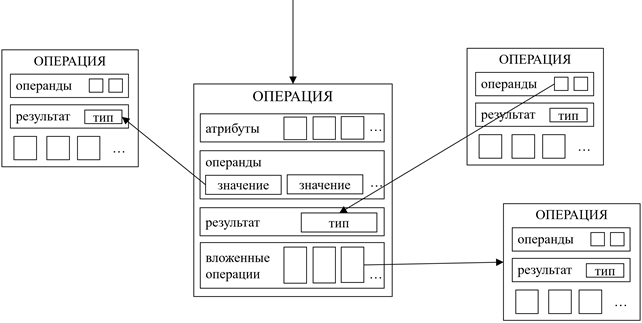
\includegraphics[width=\textwidth]{images/optree-scheme.png}
    \caption{Дерево операций.}
    \label{fig:optree_scheme}
\end{figure}

\textbf{Операция} владеет внешними значениями (результатами) и внутренними регистрами.
Результаты видны соседям операции и могут быть операндами других операций, но не видны операциям внутри тела.
Внутренние регистры, наоборот, доступны для использования операциями внутри тела, но снаружи не видны (как переменные во вложенном блоке в C++).
Операция не владеет операндами, так как это результаты или внутренние регистры других операций.
Также внутри хранится имя операции и код, определяющий ее вид.

\textbf{Значение} -- это единоразово определяемый неизменяемый регистр (как const переменная в C++).
Значение нельзя “изменить”, но можно создать новую операцию, которая будет иметь нужное значение в качестве результата, а старое значение отбросить (при необходимости удалить порождающую его операцию из дерева).
Значение хранит внутри себя породившую операцию, тип, список использований (операций, среди операндов которых есть указанное значение).

\textbf{Тип} -- это характеристика представления значения; неизменяемая структура, содержащая информацию, полезную для, собственно, представляемого типа.
Система типов в дереве операций сходна с системой типов компилируемого языка.

\textbf{Атрибут} -- это вспомогательные данные, которые используются для анализа операции (какое-либо численное значение, тип, подвид операции, строка и так далее).
Например, операция, описывающая функцию, может иметь имя функции и тип в качестве атрибутов, а операция, описывающая объявление константы - значение и тип константы и т. д.

К особенностям дерева операций можно отнести следующее:

\begin{itemize}
    \item Дерево операций можно построить из синтаксического дерева за один проход.
    \item Анализ использования значения представляет собой обход готового списка.
    \item Добавление или изменение операций прозрачно: операция хранит информацию о своем положении в дереве, значение хранит информацию о связанной операции и типе.
    \item Невозможно восстановить текст исходной программы напрямую, но можно ссылаться на исходный код в диагностике для пользователя, если сохранить ссылки на места в коде внутри операций при их создании из улов синтаксического дерева.
\end{itemize}

Для перевода синтаксического дерева в дерево операций был разработан модуль «конвертер».
Принцип работы конвертера, то есть, построения дерева операций состоит в обходе синтаксического дерева и создании операций в соответствии с типом и структурой узла синтаксического дерева с помощью вспомогательной инфраструктуры для вставки узлов.

\subsection{SSA}

SSA...
